\begin{figure}[h!]
    \centering
    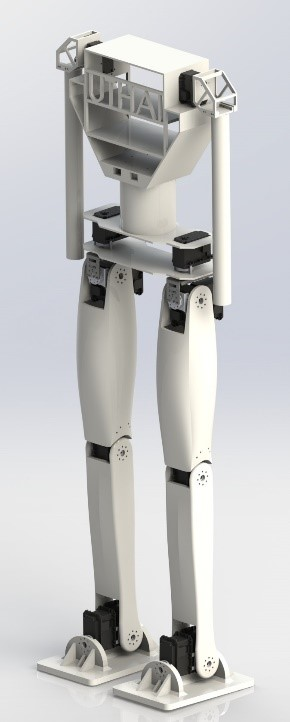
\includegraphics[width=0.2\textwidth]{chapter4/images/UTHAI_ver_1.jpg}
    \caption{โครงสร้างหุ่นยนต์ในโปรแกรม 3 มิติ}
    \label{fig:UTHAI_ver_1}
\end{figure}

โครงสร้างของหุ่นยนต์หลักๆจะแบ่งออกเป็น 2 ส่วนคือ ส่วนท่อนบนและส่วนท่อนล่างโดยส่วนท่อนบนจะประกอบไปด้วย 
เอว 1 ส่วน ลำตัว 1 ส่วน แขน 2 ส่วน และท่อนล่างจะประกอบไปด้วย สะโพก 1 ส่วน ขา 2 ส่วน น่อง 2 ส่วน ฝ่าเท้า 2 ส่วน 
ในการเลือกใช้วัสดุนั้นได้แสดงในตาราง 4.2

\begin{table}[ht]
	\centering
	\begin{tabular}{| l | l |}
		\hline
		ชิ้นส่วน & วัสดุที่ใช้ขึ้นรูป \\
        \hline
        แขน	& ท่อคาร์บอนไฟเบอร์ ขนาด 30 มม. \\
        ลำตัว & เครื่องพิมพ์ 3 มิติ โดยใช้วัสดุ PLA \\
        เอว	& ท่อคาร์บอนไฟเบอร์ ขนาด 88 มม. \\
        สะโพก & อลูมิเนียมอัลลอยพับ \\
        น่อง & เครื่องพิมพ์ 3 มิติ โดยใช้วัสดุ PLA \\
        ขา & เครื่องพิมพ์ 3 มิติ โดยใช้วัสดุ PLA \\
        ฝ่าเท้า	& เครื่องพิมพ์ 3 มิติ โดยใช้วัสดุ PLA \\
	    \hline
	\end{tabular}
	\caption{ตารางแสดงวัสดุที่ใช้ขึ้นรูป UTHAI}
	\label{tab:UTHAI_material}
\end{table}

\clearpage
\subsection{การออกแบบขา}
\subsubsection*{การออกแบบโครงสร้างส่วนขา(ครั้งที่1)}
การออกแบบโครงสร้างส่วนขาของหุ่นยนต์ฮิวมานอยด์ ได้ออกแบบโดยคำนึงถึงการขึ้นรูปด้วยเครื่องพิมพ์สามมิติ (3D Printer) 
แต่เนื่องจากว่าเครื่องพิมพ์สามมิติที่ใช้ในการผลิตนั้นมีขนาดที่เล็กกว่าขนาดที่จะพิมพ์จริงจึงต้องทำการแยกส่วนของขาออก
เป็นจำนวน 2 ส่วนในแต่ละในก้านต่อของขาท่อนบนและขาท่อนล่าง และหลังจากนั้นใช้การยึดชิ้นส่วนด้วยการตอกสลักเพื่อยึดติดชิ้นส่วนเข้าด้วยกัน
เพื่อให้มีความแข็งแรงมากกว่าการต่อแบบทั่วไป

\begin{figure}[h!]
    \centering
    \begin{subfigure}[b]{0.3\linewidth}
      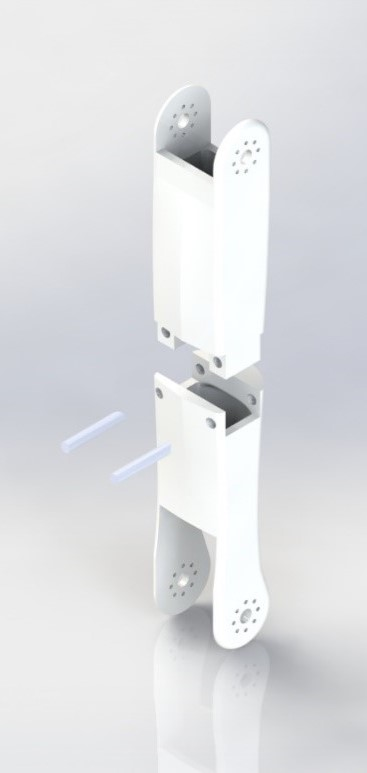
\includegraphics[width=\linewidth]{chapter4/images/shin.jpg}
      \caption{โครงสร้างส่วนหน้าแข้ง}
    \end{subfigure}
    \begin{subfigure}[b]{0.35\linewidth}
      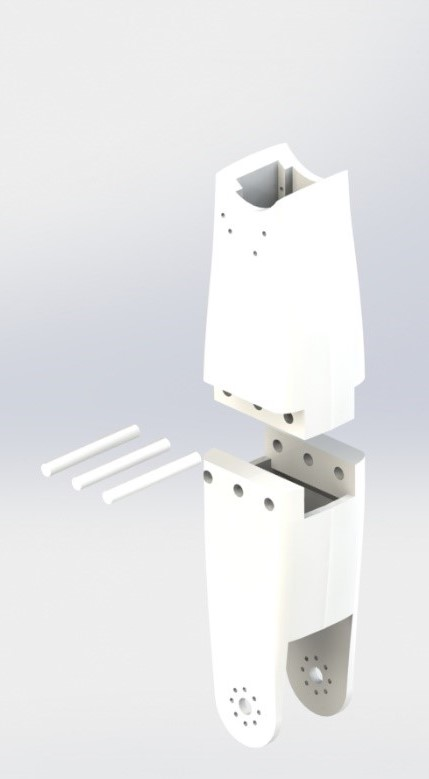
\includegraphics[width=\linewidth]{chapter4/images/thigh.jpg}
      \caption{โครงสร้างส่วนต้นขา}
    \end{subfigure}
    \caption{รูปการออกแบบส่วนขาของหุ่นยนต์อุทัย}
    \label{fig:leg}
  \end{figure}

เมื่อทำการพิมพ์ชิ้นงานส่วนขาท่อนบนและท่อนล่าง ออกมาจะได้น้ำหนักของชิ้นงานตามตาราง \ref{tab:UTHAI_leg}
\begin{table}[ht]
	\centering
	\begin{tabular}{| l | l |}
		\hline
		ชิ้นส่วน & น้ำหนัก(กรัม) \\
        \hline
        ต้นขา & 263 \\
        หน้าแข้ง & 204 \\
	    \hline
	\end{tabular}
	\caption{ตารางแสดงน้ำหนักของชิ้นส่วนขา}
	\label{tab:UTHAI_leg}
\end{table}

จากการทดสอบความสามารถในการเคลื่อนที่ พบว่าตัวขับเคลื่อนสามารถเคลื่อนที่เข้าตำแหน่งได้ถูกต้องตามมุม 
ที่ป้อนเข้าไปให้ระบบ แต่หากทำให้ชิ้นส่วนของขาเคลื่อนที่ด้วยถี่ไปกลับสูงและด้วยความเร็วที่มาก จะทำให้ตัวขับเคลื่อนเกิดการโอเวอร์โหลด 
ซึ่งมีผลทำตัวขับเคลื่อนหยุดการทำงาน ซึ่งต้องทำการปิดเปิดตัวขับเคลื่อนใหม่

\clearpage
\subsubsection*{ผลการทดสอบ}
จากการทดสอบความแข็งแรงของชิ้นงาน พบว่าชิ้นงานมีความแข็งแรงเพียงพอที่จะทำให้ตัวขับเคลื่อนมีค่าแรงบิดเป็นค่าแรงบิดสูงสุด(Stall Torque)
แล้วทำให้ชิ้นงานไม่เกิดความเสียหาย

จากการทดสอบระยะเวลาการทำงานของตัวขับเคลื่อน ด้วยการเขียนโปรแกรมให้ตัวขับเคลื่อน เคลื่อนที่ไปกลับ สลับตำแหน่งไปเรื่อยๆอย่างต่อเนื่อง เป็นเวลา 20 นาที
พบว่า ตัวขับเคลื่อนทำงานได้เป็นปกติ

\subsubsection*{ปัญหาที่พบในการออกแบบครั้งที่ 1}
เนื่องจากว่าเป้าหมายของการสร้างหุ่นยนต์ตัวนี้ให้มีน้ำหนักที่เบา (น้อยกว่า 5 กิโลกรัม) จึงพบปัญหาว่า
น้ำหนักของส่วนขาที่ได้ออกแบบมานั้นมีน้ำหนักมากเกินกว่าของหุ่นยนต์กนก(ชื่อหุ่นยนต์ตัวเดิมก่อนจะเป็นอุทัย)
ซึ่งเป็นผลทำให้เกิดปํญหาเรื่องภาระโหลดของ motor ที่ต้องกระทำที่มีมากขึ้นจากเดิมและจะทำให้น้ำหนักของตัวหุ่นยนต์มากขึ้น 
เมื่อเปรียบเทียบผลลัพธ์น้ำหนักส่วนขาของหุ่นยนต์กนกกับหุ่นยนต์อุทัยแล้วได้ผลดังตาราง \ref{tab:UTHAI_KANOK_Comp}

\begin{table}[ht]
	\centering
	\begin{tabular}{| l | l | l |}
		\hline
        ชิ้นส่วน & หุ่นยนต์กนก(เดิม)(กรัม) & หุ่นยนต์ UTHAI \\
        \hline
        ขาท่อนบน & 171 & 263 \\
        ขาท่อนล่าง & 172 & 204 \\
	    \hline
	\end{tabular}
	\caption{ตารางเปรียบเทียบน้ำหนักของชิ้นส่วนขาของหุ่นยนต์}
	\label{tab:UTHAI_KANOK_Comp}
\end{table}

จากข้อมูลในตารางนั้นจะเห็นได้ว่า หนักที่เพิ่มขึ้นมากจากการออกแบบใหม่แต่ละชิ้นนั้น มากถึง 124 กรัม
ต่อขา 1 ข้าง และ 248 กรัมเมื่อเทียบกับขาทั้งหมดและเปรียบเทียบกับข้อมูลก่อนหน้า

หลังจากพบปัญหาดังกล่าวผู้จัดทำจึงได้ตัดสินใจทำการเปลี่ยนวัสดุที่ใช้ทำโครงสร้างในครั้งแรก
ที่จะใช้การขึ้นรูปชิ้นงานด้วยการพิมพ์ขึ้นรูป 3 มิติ มาเป็นวัสดุผลระหว่างคาร์บอนไฟเบอร์และชิ้นงาน 3 มิติแทน
โดยจะให้ชิ้นงาน 3 มิตินั้นทำหน้าที่เป็นตัวเชื่อมระหว่างวัสดุคาร์บอนไฟเบอร์กับมอเตอร์ และยึดกับวัสดุคาร์บอนไฟเบอร์ด้วยการบีบ
ซึ่งเหตุผลที่ต้องทำเช่นนี้เพราะต้องการลดน้ำหนักของหุ่นยนต์ลง เพื่อไม่ให้มอเตอร์รับภาระที่หนักเกินไป 

\begin{table}[ht]
	\centering
	\begin{tabular}{| l | l | l |}
		\hline
		ชิ้นส่วน & วัสดุที่ใช้ขึ้นรูป(เก่า) & วัสดุที่ใช้ขึ้นรูป(ใหม่) \\
        \hline
        แขน	& ท่อคาร์บอนไฟเบอร์ ขนาด 30 มม. & เดิม\\
        ลำตัว & เครื่องพิมพ์ 3 มิติ โดยใช้วัสดุ PLA & เดิม\\
        เอว	& ท่อคาร์บอนไฟเบอร์ ขนาด 88 มม. & เดิม\\
        สะโพก & อลูมิเนียมอัลลอยพับ & เดิม\\
        น่อง & เครื่องพิมพ์ 3 มิติ โดยใช้วัสดุ PLA & วัสดุผสมระหว่างคาร์บอนไฟเบอร์และ ชิ้นงาน 3 มิติ \\
        ขา & เครื่องพิมพ์ 3 มิติ โดยใช้วัสดุ PLA  & วัสดุผสมระหว่างคาร์บอนไฟเบอร์และ ชิ้นงาน 3 มิติ\\
        ฝ่าเท้า	& เครื่องพิมพ์ 3 มิติ โดยใช้วัสดุ PLA & เดิม\\
	    \hline
	\end{tabular}
	\caption{ตารางแสดงวัสดุที่แก้ไขในการใช้ขึ้นรูป UTHAI }
	\label{tab:UTHAI_materialchange}
\end{table}

\clearpage
\subsubsection*{การออกแบบโครงสร้างส่วนขา(ครั้งที่2)}
ครั้งนี้การออกแบบชิ้นส่วนขาของหุ่นยนต์นั้น ได้คำนึงถึงเรื่องน้ำหนักเป็นหลัก และยังคงให้ความสำคัญกับข้อต่อที่จะใช้รับน้ำหนักทั้งตัวหุ่นยนต์
และยังคงรับแรงบิดของมอเตอร์อีกด้วย ดังนั้นจึงได้ตัดสินใจที่จะเปลี่ยนจากการใช้วัสดุ 3D print  ซึ่งเป็นพลาสติกทั้งหมด มาเป็นวัสดุผสม 
ระหว่าง Carbonfiber กับ 3D print ซึ่งขึ้นรูปจากพลาสติก PLA และทำการยึดติดกันด้วยการบีบอัดดังรูปที่\ref{fig:newleg}
เมื่อทำการพิมพ์ชิ้นงานส่วนขาท่อนบนและท่อนล่างและทำการประกอบ จะได้น้ำหนักของชิ้นงานเปรียบเทียบกับของเดิมดังตามตาราง\ref{tab:UTHAI_leg_compilation}

\begin{figure}[h!]
    \centering
    \begin{subfigure}[b]{0.3\linewidth}
      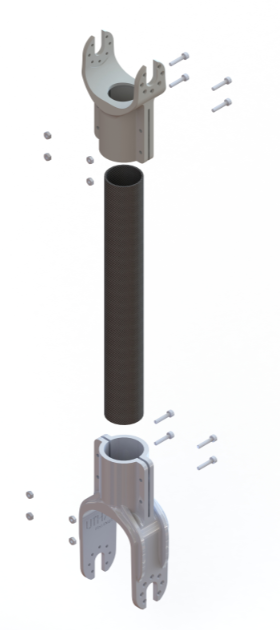
\includegraphics[width=\linewidth]{chapter4/images/carb_shin.png}
      \caption{โครงสร้างส่วนหน้าแข้ง(ใหม่)}
    \end{subfigure}
    \begin{subfigure}[b]{0.3\linewidth}
      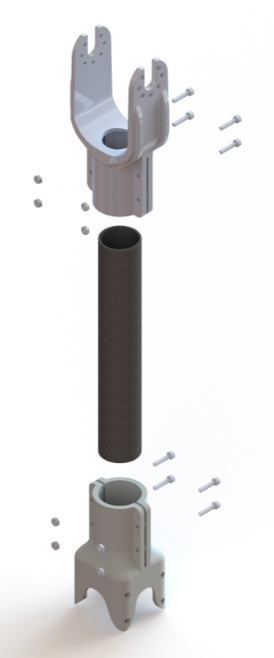
\includegraphics[width=\linewidth]{chapter4/images/carb_thigh.png}
      \caption{โครงสร้างส่วนต้นขา(ใหม่)}
    \end{subfigure}
    \caption{รูปการออกแบบส่วนขาของหุ่นยนต์อุทัย(ใหม่)}
    \label{fig:newleg}
  \end{figure}

\begin{table}[h!]
	\centering
	\begin{tabular}{| l | l | l |}
		\hline
		ชิ้นส่วน & น้ำหนักเดิม(กรัม) & น้ำหนักใหม่(กรัม) \\
        \hline
        ต้นขา & 263 & 161\\
        หน้าแข้ง & 204 & 166\\
	    \hline
	\end{tabular}
	\caption{ตารางแสดงน้ำหนักเปรียบเทียบของชิ้นส่วนขา}
	\label{tab:UTHAI_leg_compilation}
\end{table}  

\clearpage
\subsubsection*{การขึ้นรูปชิ้นงาน}
การขึ้นรูปชิ้นงานนนั้น ได้ใช้การขึ้นรูปชิ้นตามความสูงแนวแกน Z ดังภาพ \ref{fig:print_axis} เพื่อให้ชิ้นงานมีความสวยงามและสามารถสวมได้พอดี
กับท่อนคาร์บอนโดยให้มีผิวสัมผัสมากที่สุด ในการยึดเกาะ\footnote{Experimental Characterization of the Mechanical Properties of 3D-Printed ABS and Polycarbonate Parts}
\begin{figure}[h!]
    \centering
    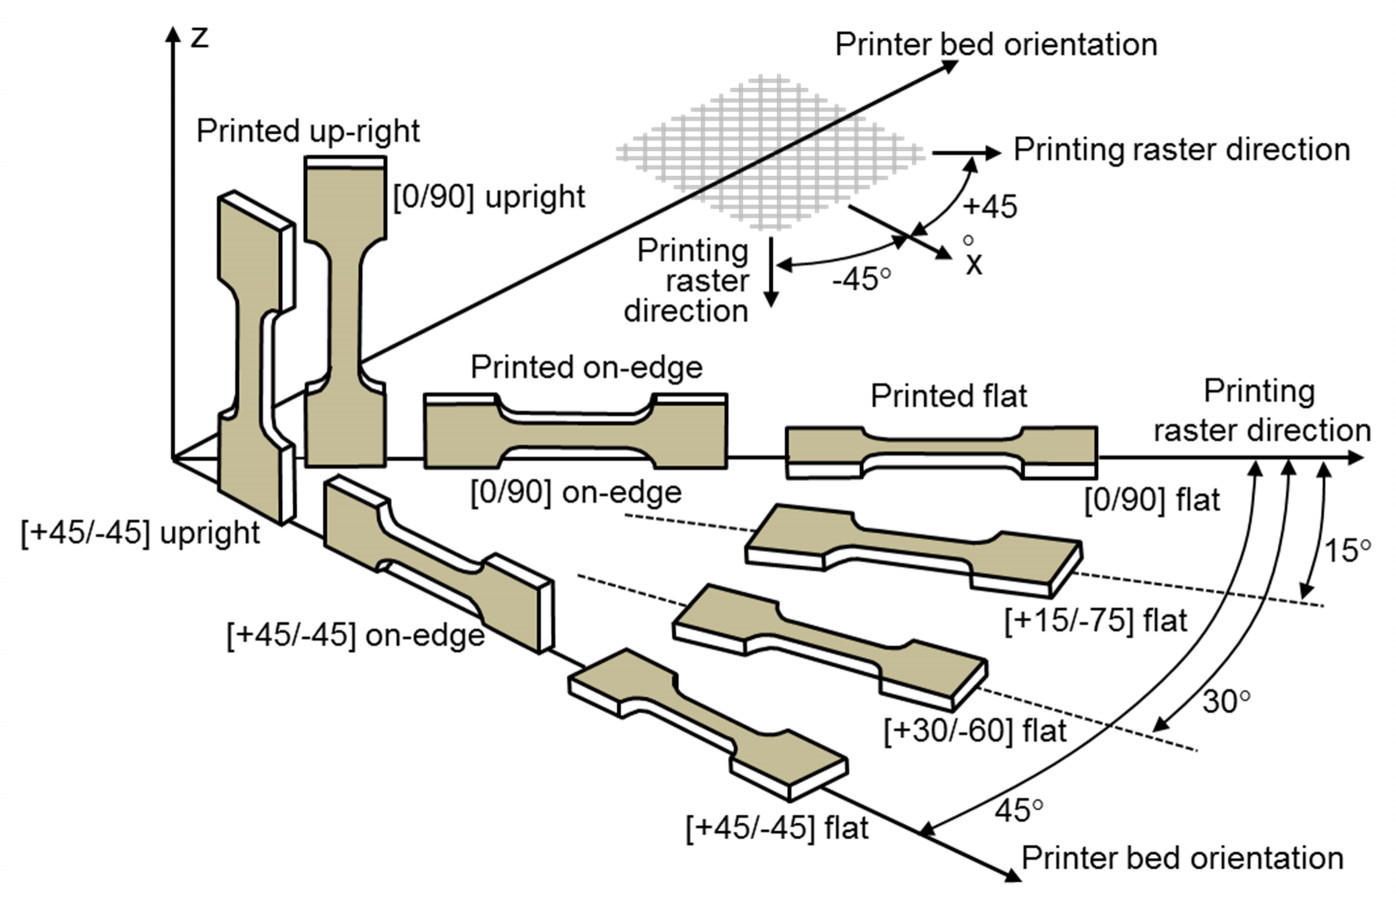
\includegraphics[width=0.6\textwidth]{chapter4/images/print_axis.png}
    \caption{รูปการชิ้นรูปชิ้นงานของ 3D printer }
    \label{fig:print_axis}
\end{figure}

\subsubsection*{ทดสอบโครงสร้างและการขับเคลื่อน}	
จากการทดสอบความแข็งแรงของวัสดุโดยการนำไปประกอบกับตัวหุ่นยนต์จริง และทำการทดลองเดินพบว่าเมื่อทำการเดินจริงนั้น 
เกิดการฉีกขาดของชิ้นงานที่ ชั้นการพิมพ์ของชิ้นงานดังภาพ 4.9 ซึ่งเกิดจากการได้รับแรงบิดมากเกินไปจากน้ำหนักของชิ้นงานส่วนขา
และแรงที่ชิ้นงานจะได้รับนั้น จะเป็นเพียงส่วนการเชื่อมกันติดของชั้นพลาสติกเท่านั้น ซึ่ง ณ ที่นี้เส้นพลาสติกจะไม่ได้เป็นตัวรับแรงจึงทำให้
เกิดการเปราะหักที่ง่ายกว่าดังนั้นจึงทำการออกแบบใหม่โดยการเพิ่มสันให้ชิ้นงานและเพื่มความหนาบนหน้าแปลนเชื่อมกับตัวมอเตอร์
และทำการขึ้นรูปชิ้นงาน โดยให้ความสูงของชิ้นงานเป็นไปตามแกน X และทำการเติมเนื้อพลาสติกด้านในให้เต็ม 100\% ดังรูปที่ \ref{fig:fatiguelayer}
\begin{figure}[h!]
    \centering
    \begin{subfigure}[b]{0.2\linewidth}
      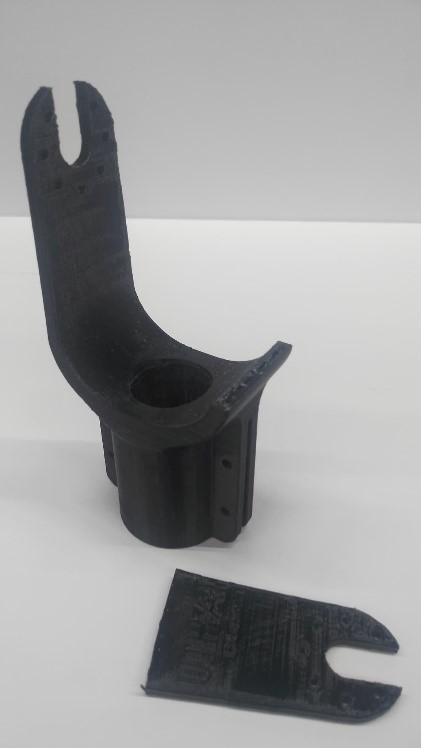
\includegraphics[width=\linewidth]{chapter4/images/fatigue1.jpg}
      \caption{รูปแสดงการแตกหักของชิ้นงาน}
    \end{subfigure}
    \begin{subfigure}[b]{0.3\linewidth}
      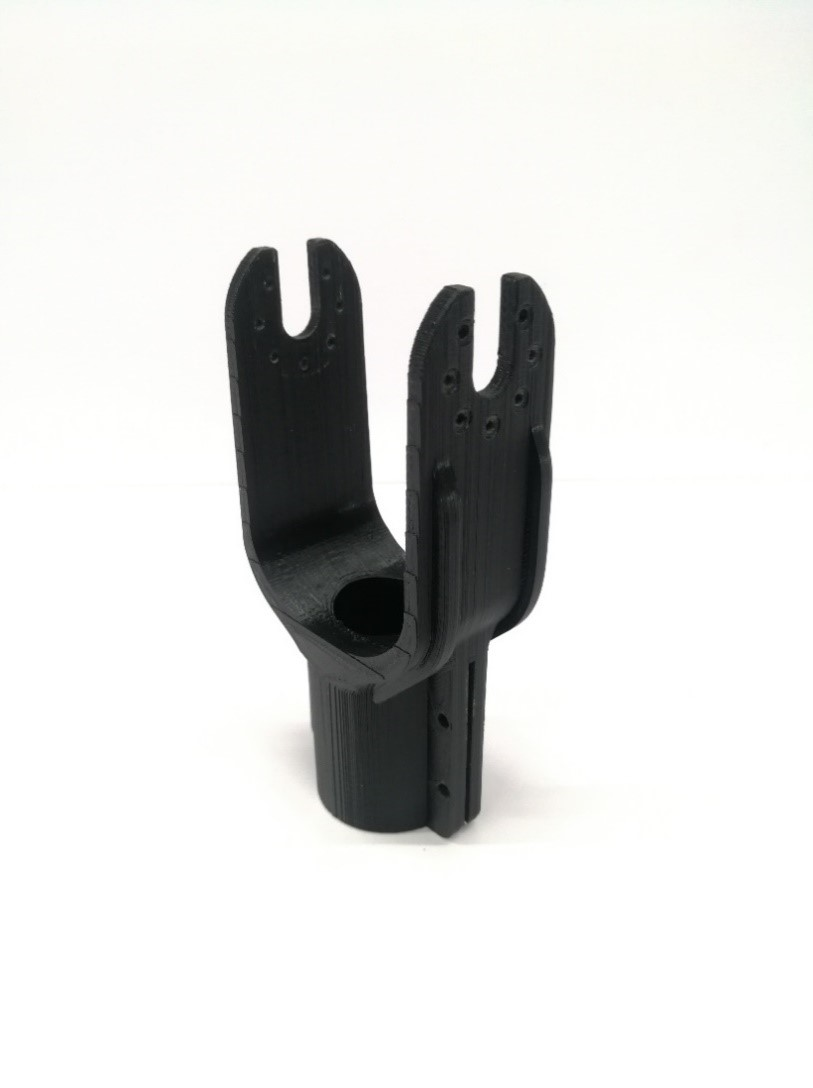
\includegraphics[width=\linewidth]{chapter4/images/fatigue2.jpg}
      \caption{รูปแสดงชิ้นงานที่ทำการออกแบบใหม่}
    \end{subfigure}
    \begin{subfigure}[b]{0.4\linewidth}
        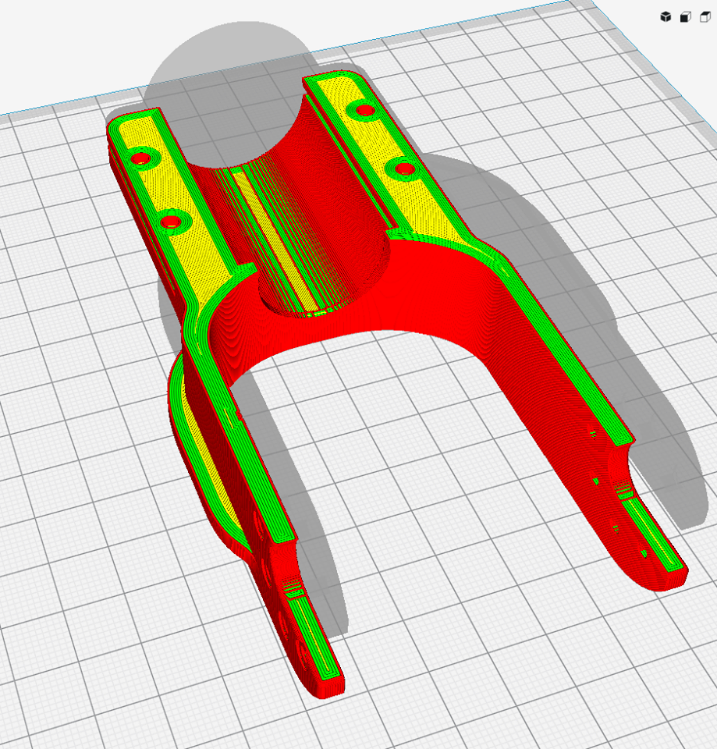
\includegraphics[width=\linewidth]{chapter4/images/fatigue3.png}
        \caption{รูปแสดงชั้นของการพิมพ์โดยการเติมเนื่อพลาสติก 100\%}
    \end{subfigure}
    \caption{รูปแสดงการแตกหักและชั้นการพิมพ์}
    \label{fig:fatiguelayer}
  \end{figure}

\subsubsection*{การทดลองความแข็งแรงของชิ้นงานโดยวิธีการวิเคราะห์เชิงตัวเลข(Finite element)}
ก่อนที่จะนำชิ้นงานที่ทำการออกแบบใหม่ที่เติมเนื่อพลาสติก 100\% ไปใช้งานจริงนั้นจะต้องผ่านการวิเคราะห์แรงกระทำ
โดยผ่านโปรแกรมจำลองเพื่อหาจุดที่เปราะบางของชิ้นงาน  และนำข้อมูลนั้นไปวิเคราะห์เพื่อปรับปรุงชิ้นงานต่อไป 
ซึ่งได้ตั้งค่า คุณสมบัติของชิ้นงาน 3d print ไว้ดังนี้ 
\begin{table}[ht]
	\centering
	\begin{tabular}{| l | l |}
		\hline
		Print Orientation Side	& flat \\
        \hline
        Ultimate Stress$(N/mm²)$\footnote{Tensile Testing of 3D Printed Materials for Scoliosis Brace( Rahul Malik)} & 	45.66 \\
        Young’s Modulus$(N/mm²)$\footnote{Tensile Testing of 3D Printed Materials for Scoliosis Brace( Rahul Malik)} & 	1141.55 \\
        Yield strength$(N/mm²)$\footnote{What is the influence of infill \%, layer height and infill pattern on my 3D prints (3D Matter)} & 23 \\
        Density$(kg/m^3)$\footnote{Filament volume and length(toybuilderlabs)} &	1250 \\
        Passion ratio\footnote{Additive Manufacturing and Characterization of Polylactic Acid (PLA) Composites ContainingMetal Reinforcements(NASA)} &	0.33 \\
        Force(torque)$(N.m)$ & 10.4 \\
	    \hline
	\end{tabular}
	\caption{ตารางแสดงค่าคุณสมบัติของวัสดุ 3D print(PLA)}
	\label{tab:PLA_property}
\end{table}

เมื่อทำการวิเคราะห์ผ่านโปรแกรม solidword ได้ผลลัพธ์ ดังนี้

\begin{figure}[h!]
  \centering
  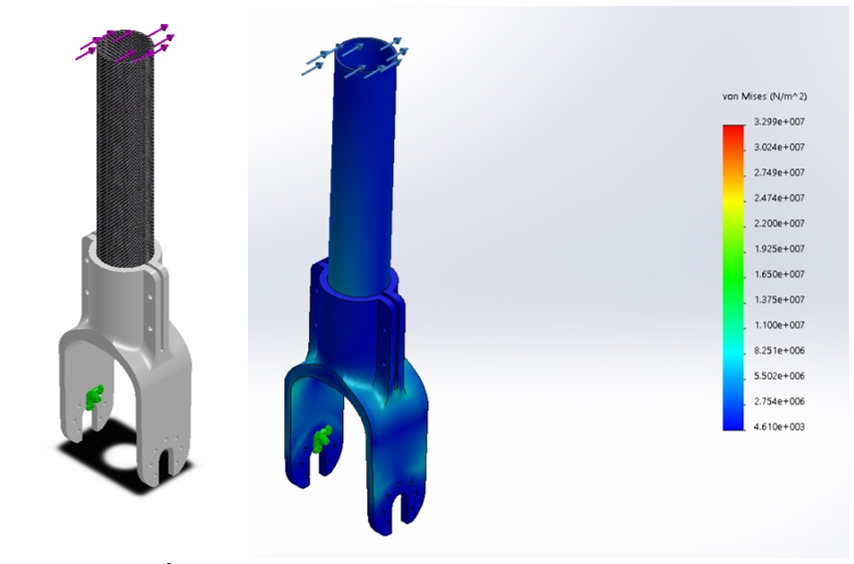
\includegraphics[width=0.8\textwidth]{chapter4/images/FEA1.png}
  \caption{รูปการวิเคราะห์แรงของข้อต่อ 1}
  \label{fig:FEAjoint1}
\end{figure}

\clearpage
\begin{figure}[h!]
  \centering
  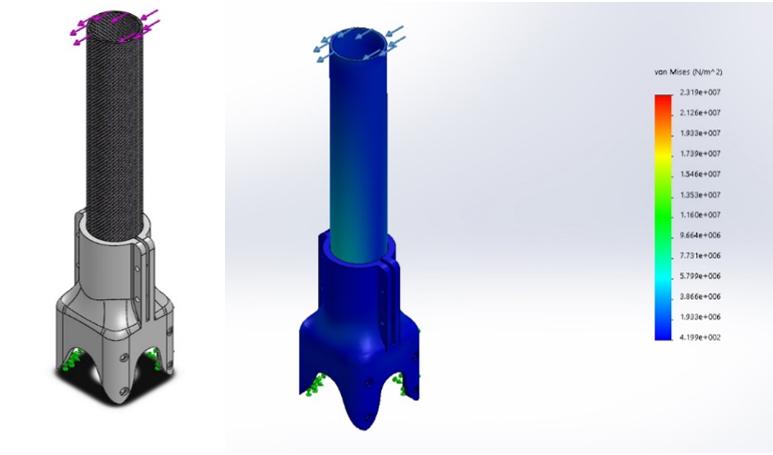
\includegraphics[width=0.8\textwidth]{chapter4/images/FEA2.png}
  \caption{รูปการวิเคราะห์แรงของข้อต่อ 2}
  \label{fig:FEAjoint2}
\end{figure}

\begin{figure}[h!]
  \centering
  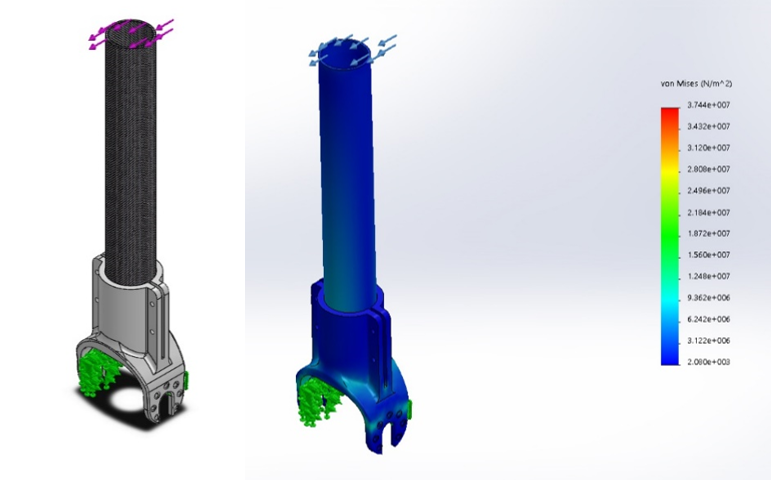
\includegraphics[width=0.8\textwidth]{chapter4/images/FEA3.png}
  \caption{รูปการวิเคราะห์แรงของข้อต่อ 3}
  \label{fig:FEAjoint3}
\end{figure}
\clearpage

การวิเคราะห์นั้นจะทำการยึดจุดที่เป็นหน้าแปลนของมอเตอร์ไว้เพื่อให้เปรียบเสมือนกับว่าขณะนี้ชิ้นงาน
ได้เชื่อมติดกับตัวมอเตอร์ หลังจากนั้นกำหนดแรงกระทำเพื่อให้เกิดโมเมนต์กับชิ้นงานโดยค่าแรงที่กระทำนั้น
ได้มาจากการคำณวนแรงของมอเตอร์ที่จะรับไหวเทียบกับระยะของแรง ที่กระทำกับชิ้นงาน 
ซึ่งได้ทดลองกับชิ้นงานตัวข้อต่อ 1 2 และ 3 ด้วยแรง 41.6 นิวตัน$(N)$
เมื่อนำค่า ความตึงเครียดสูงสุด$(Max stress)$ของชิ้นงานมาวิเคราะห์เพื่อหา จุดเปราะบางของวัสดุได้ค่าดังตาราง
\ref{tab:streaa_result}
\begin{table}[ht]
	\centering
	\begin{tabular}{| l | c |}
		\hline
		ชื่อชิ้นงาน	& ความตึงเครียดสูงสุดของชิ้นงาน(Max stress)$(N/mm^2)$ \\
        \hline
        ข้อต่อ 1 & 32.99 \\
        ข้อต่อ 2 & 23.19 \\
        ข้อต่อ 3 & 7.987 \\
	    \hline
	\end{tabular}
	\caption{ตารางแสดงความตึงเครียดของชิ้นงาน(Stress)}
	\label{tab:streaa_result}
\end{table}

จากผลการทดลองสรุปได้ว่า ค่าความตึงเครียดต่างๆที่ได้มาจากผลลัพธ์นั้นเมื่อนำไปเทียบกับค่าความตึงเครียดสูงสุดที่วัสดุจะรับไหว
ที่ 45.66 N/mm² เห็นได้ว่ายังคงไม่มีวัสดุตัวไหนที่จะเกิดการแตกหักเมื่อเกิดแรงกระทำกับชิ้นงานดังนั้นชิ้นงานที่ทำการออกแบบนี้
พอสรุปได้ว่าจะไม่เกิดการแตกหักระหว่างการทำงาน ยกแว้นมีแรงกระทำจากภายนอกที่มากเกินไปจนมาผลทำให้เกิดความตึงเครียดของชิ้นงานสูง
เกินกว่าค่าดังกล่าว  

\subsection{การออกแบบเท้า}
............
\subsubsection{เซนเซอร์ตรวจจับการสัมผัสพื้น}
แนวคิดการออกแบบหลัก คือการออกแบบให้สามารถติดตั้งกับตัวหุ่นยนต์ได้เลย ไม่ต้องเชื่อมต่อสายไฟและสายส่งข้อมูลใหม่ โดยให้ใช้สายไฟไฟเลี้ยง 
และสายสัญญาณชุดเดียวกับตัวขับเคลื่อน Dynamixel Servo Mo-tor ซึ่งมีการติดต่อกันในลักษณะเป็นบัสแบบ RS-485 ดังนั้นแล้วผู้เขียนจึงเลือกที่จะทำโมดูลขึ้นมาใหม่ 1 โมดูล 
เพื่อที่ใช้ในการอ่านค่า Ground Contact Sensor ของหุ่นยนต์โดยเฉพาะ โดยมีการติดต่อรูปแบบบัส RS-485 ใช้ลักษณะการติดต่อสื่อสาร(Protocol) เดียวกับตัวขับเคลื่อน Dynamixel 
และมีการพัฒนาจาก Arduino ซึ่งให้สามารถอ่านค่าได้ทั้ง Analog และ Digital ได้ อีกทั้งรองรับการต่อ Sensor แบบ Force sensitive resistor จำนวน 4 ตัว.

\clearpage
\begin{figure}[h!]
  \centering
  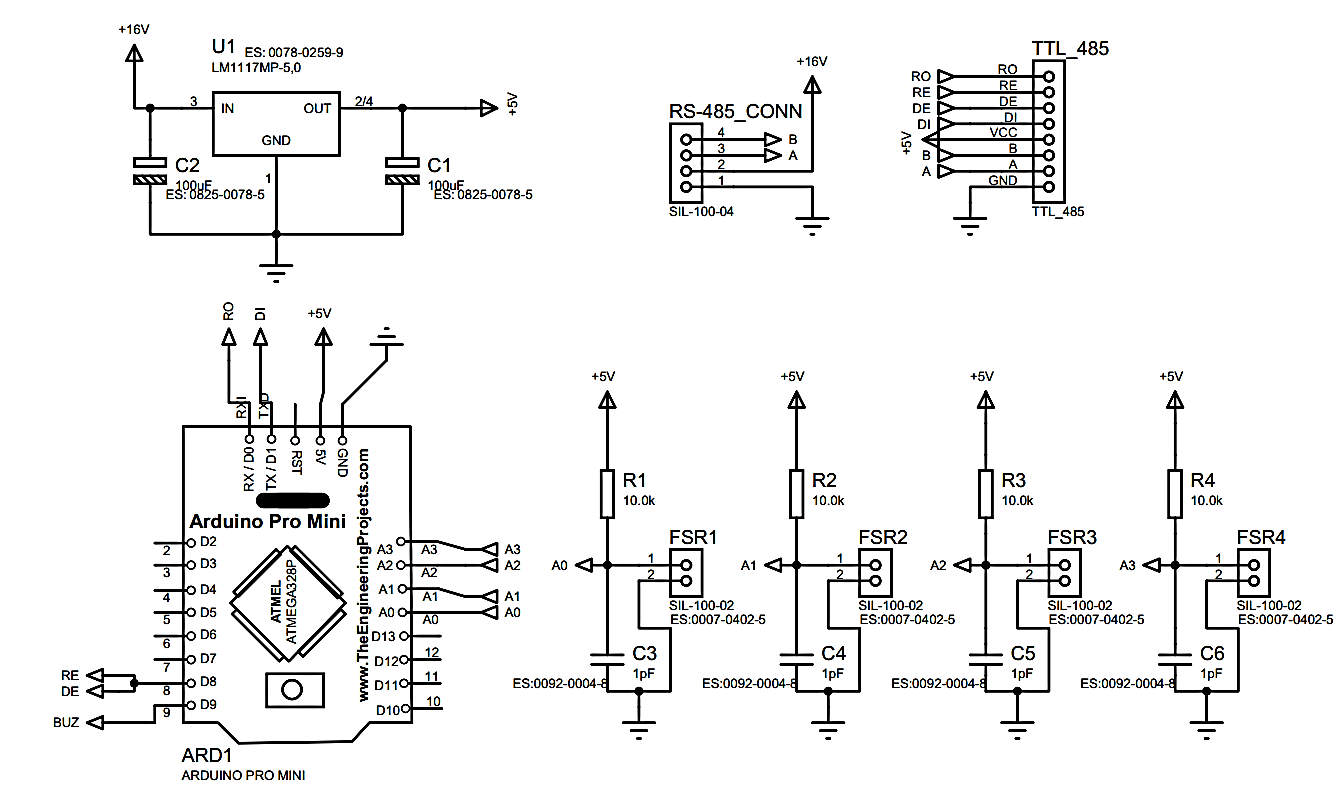
\includegraphics[width=0.8\textwidth]{chapter4/images/FSR_schematic.png}
  \caption{Schematic ของวงจร Ground Contact Sensor}
  \label{fig:FSR_schematic}
\end{figure}

\begin{figure}[h!]
  \centering
  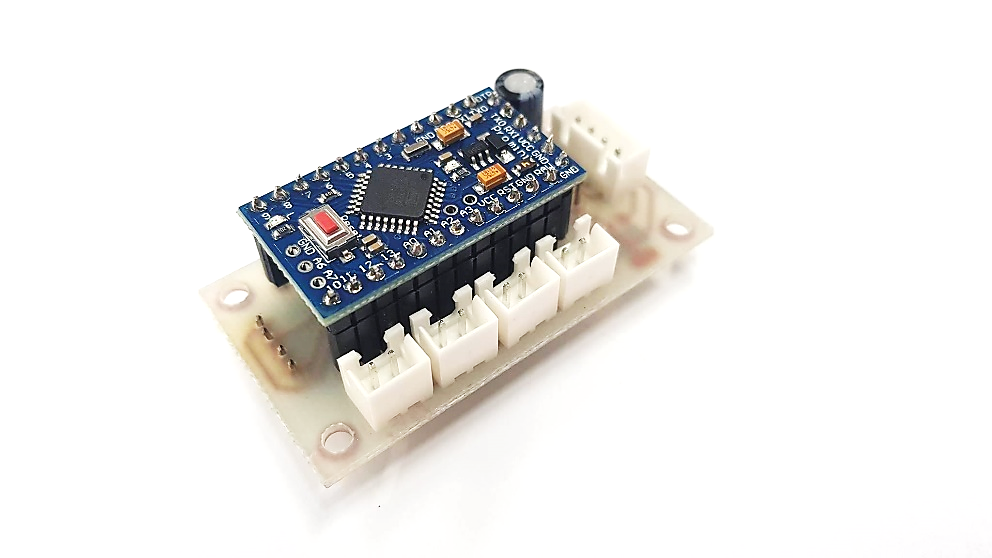
\includegraphics[width=0.8\textwidth]{chapter4/images/complete_FSR.png}
  \caption{แผงวงจร Ground Contact Sensor ที่ประกอบเสร็จแล้ว}
  \label{fig:complete_FSR}
\end{figure}

เซนเซอร์ที่เลือกใช้คือ Force Sensitive Resistor (FSR) เป็นเซนเซอร์ที่มีค่าความต้านทานภายในตัวเอง โดยเซนเซอร์นี้มีหลักการทำงานคือ 
ค่าความต้านทานทางไฟฟ้าของตัวเซนเซอร์จะเปลี่ยนแปลงเมื่อมีแรงเข้ามากระทำกับหน้าสัมผัส เมื่อมีแรงเข้ามากระทำมาก จะทำให้ค่าความต้านทานต่ำ 
หากไม่มีแรงเข้ามากระทำจะทำให้มีค่าความต้านทานสูง และเมื่อมีการนำเซนเซอร์นี้มาต่อกับตัวต้านทานที่มีค่าคงที่ ในรูปแบบของ Voltage Divider 
ดังรูปที่ \ref{fig:FSR_schematic} จะทำให้สามารถอ่านค่าแรงดันไฟฟ้าที่เปลี่ยนแปลงตามแรงที่เกิดขึ้นกับหน้าสัมผัสของเซนเซอร์ FSR ได้ 

\begin{figure}[h!]
  \centering
  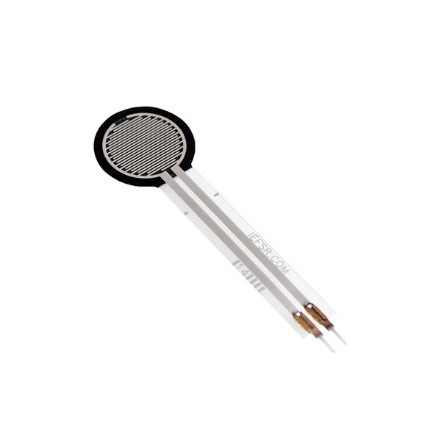
\includegraphics[width=0.4\textwidth]{chapter4/images/FSR.jpg}
  \caption{Force Sensitive Resistor (FSR) ขนาด 0.5 นิ้ว}
  \label{fig:FSR}
\end{figure}

ข้อดีของ FSR นั้นคือ เป็นเซนเซอร์ที่ถูกพัฒนาและออกแบบมาเพื่อใช้สำหรับการวัดแรงโดยตรง จึงทำให้ใช้งานได้ง่าย และสะดวก ในราคาที่ถูกกว่า 
เมื่อเทียบกับเซนเซอร์ Load cell ที่มีราคาสูงและการใช้งานจำเป็นที่จะต้องมีวงจรขยายสัญญาณที่ใช้ในการอ่านค่าการบิดของวัสดุจาก 
แต่ FSR นั้นก็มีข้อเสียเช่นกันคือ ความไม่ทนทานต่อการขีดข่วน เนื่องจากตัวเซนเซอร์ถูกทำมาจากฟิล์มพลาสติกบางๆ ซึ่งหากเกิดการขีดข่วนเกิดขึ้นแล้วอาจทำให้ฟิล์มฉีกขาดได้ 
หากฟิล์มขาดจะทำให้ค่าความต้านทานออกมาไม่เหมือนเดิม ดังนั้นทางผู้เขียนจึงเลือกที่จะออกแบบโครงครอบสำหรับเซนเซอร์ FSR เพื่อป้องกันจากการถูกขีดข่วนจากภายนอก
\begin{figure}[h!]
  \centering
  \begin{subfigure}[b]{0.4\linewidth}
    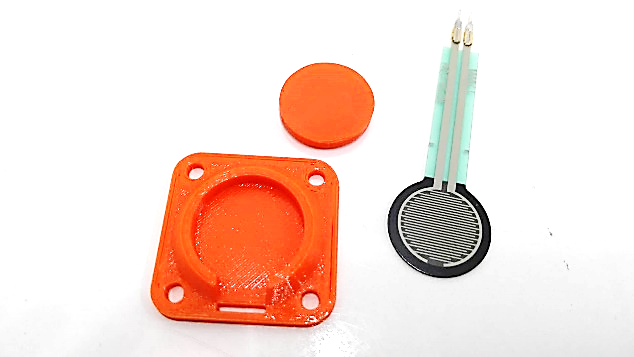
\includegraphics[width=\linewidth]{chapter4/images/FSR_cover1.png}
    %\caption{รูปแสดงการแตกหักของชิ้นงาน}
  \end{subfigure}
  \begin{subfigure}[b]{0.4\linewidth}
    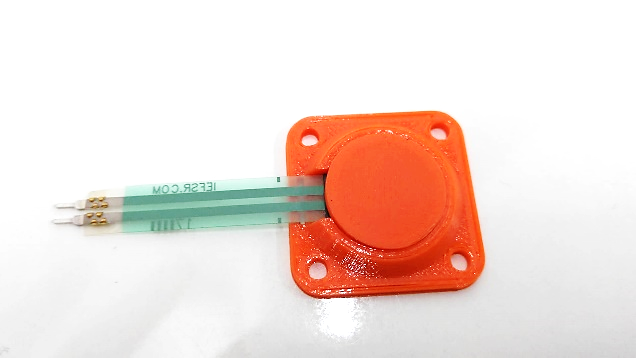
\includegraphics[width=\linewidth]{chapter4/images/FSR_cover2.png}
    %\caption{รูปแสดงชิ้นงานที่ทำการออกแบบใหม่}
  \end{subfigure}
  \caption{โครงครอบของ Force Sensitive Resistor}
  \label{fig:FSR_cover}
\end{figure}

\subsection{การออกแบบลำตัว}
\subsubsection{การติดตั้งบอร์ดควบคุมและแบตเตอรี่}

\subsection{การออกแบบแขน}



